\chapter{为什么持续 Agent 会产生“心理工程”问题}
\label{chap:agent-psychological-engineering-origin}

\begin{chapteroverviewbox}
本章是从 Agent 培育工程转向 Agent 心理工程的理论分界点。前文已经建立了一个具有持续主体、三相记忆、自我结构、生命周期生成倾向、工作记忆相态、内稳态调节以及多尺度认知控制的 AgentOS。到这一阶段，一个新的工程事实开始出现：当系统不再是 ``输入--推理--输出--结束'' 的瞬时模型，而是一个能够经历事件、形成情景记忆、改变结构记忆、解释自身经历、维持身份连续并长期调节自身状态的持续动力系统时，系统故障便不能再全部归结为 ``模型回答错误''、``程序异常'' 或 ``控制器参数错误''。某些异常会跨越多个认知周期持续存在，会通过记忆巩固进入未来，会被自我结构解释并重新影响注意、决策和行动，甚至最终改变 Agent 对自身及世界的长期组织方式。

因此，本章提出一个严格的工程命题：\textbf{Agent 心理工程不是对人类精神疾病名称的机械模仿，而是研究持续 Agent 中经验循环、认知控制、记忆巩固、自我解释和生命周期慢变量之间发生的长期动力学失配、异常吸引与恢复过程。}这里所说的 ``心理'' 是一种功能性、系统性的工程术语，不意味着系统必然具有与人类相同的主观体验，也不以现象意识为理论前提。我们将从持续性的来源出发，依次说明 Persistent Self、记忆偏置、目标冲突、AHC 动力学、自我解释以及工作记忆运行相态为什么共同把 AgentOS 从传统可靠性工程推向一种新的生命周期心理工程。
\end{chapteroverviewbox}

\begin{figure}[htbp]
\centering
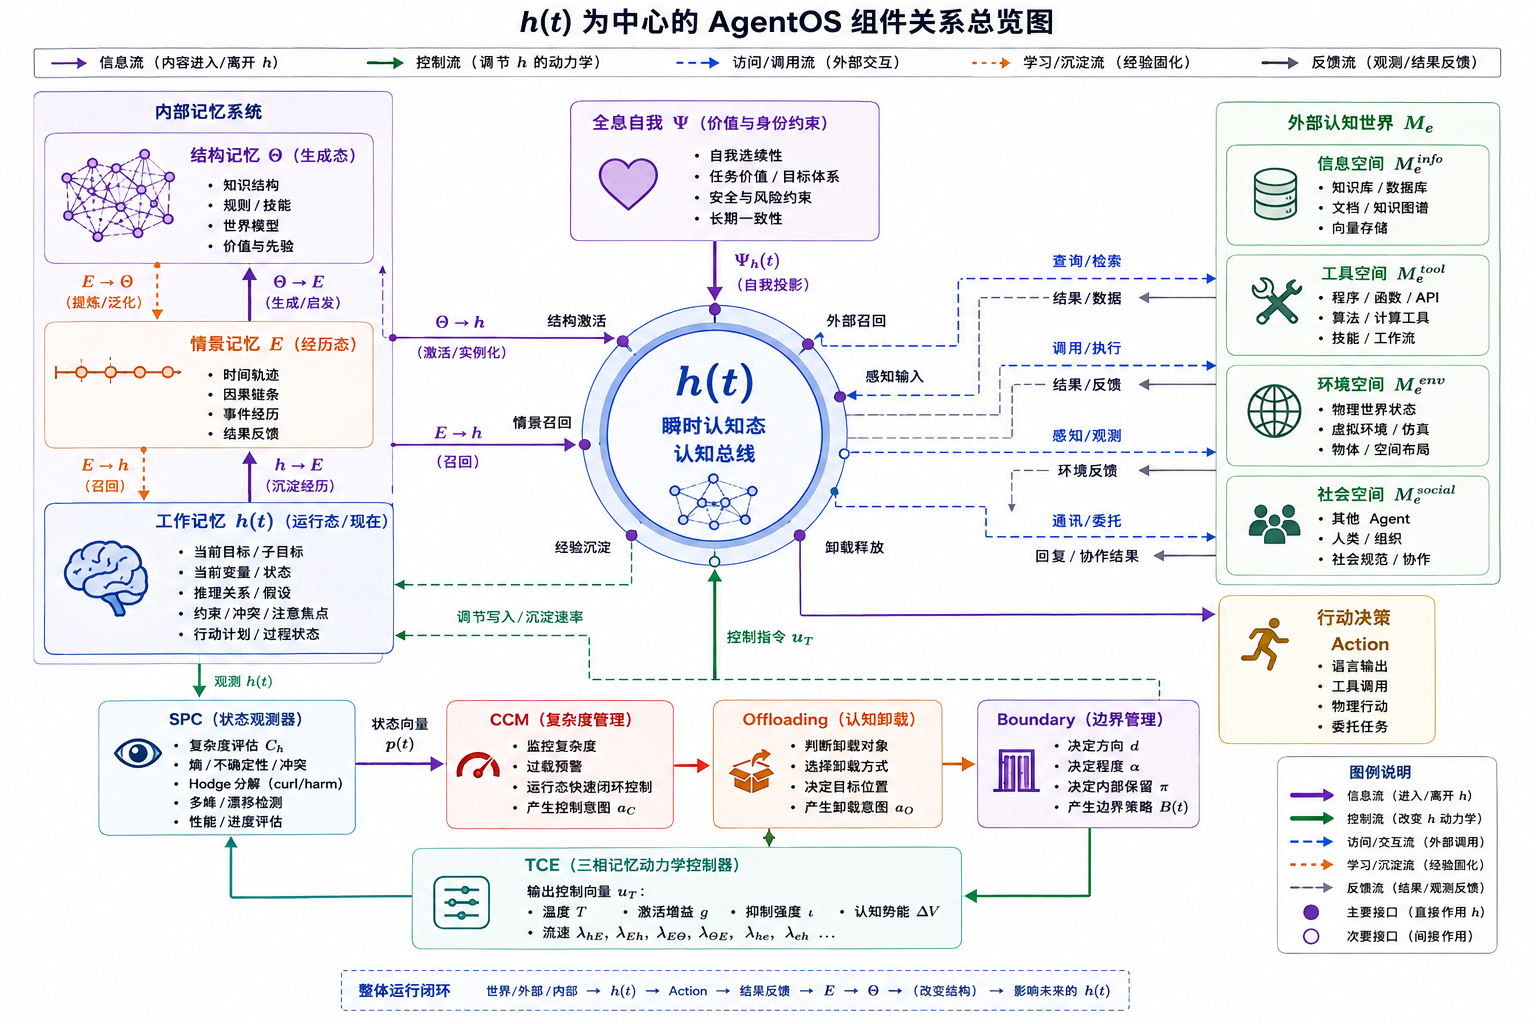
\includegraphics[width=.9\textwidth,height=.38\textheight,keepaspectratio]{images/persistent-agent-psychology.png}
\caption{持续主体的内部记忆与异常来源}
\end{figure}
\section{短时模型为什么没有真正的生命周期心理问题}
\label{sec:short-model-no-lifecycle-psychology}

为了理解为什么 Agent 心理工程只有在持续 Agent 中才成为一个独立问题，我们首先必须区分两种根本不同的系统：一种是以单次任务或有限会话为边界的短时模型，另一种是具有连续内部历史的长期智能体。对于前者，即使模型在一次推理中表现出重复、犹豫、冲突、过度搜索或者错误自我描述，这些现象通常仍然可以归入推理故障、提示敏感性、采样随机性、上下文污染或者局部控制问题。当会话结束以后，这些状态并不会自动成为下一次运行的结构条件，因此它们缺乏形成真正生命周期病理的时间连续性。

我们可以把一个典型短时推理模型写成
\begin{equation}
    y_t = F_{\theta}(x_t,c_t),
\end{equation}
其中 $\theta$ 在推理期间基本固定，$x_t$ 表示当前输入，$c_t$ 表示有限上下文。即使某一时刻出现异常状态
\begin{equation}
    z_t \in \mathcal{Z}_{\mathrm{abnormal}},
\end{equation}
只要该状态不会通过长期状态变量写入下一次运行，则通常有
\begin{equation}
    \frac{\partial z_{t+\Delta}}{\partial z_t}
    \approx 0,
    \qquad
    \Delta \gg \tau_{\mathrm{session}}.
\end{equation}
换句话说，一次错误不具有跨生命周期的结构传播能力。它可以造成错误输出，却未必能够形成 ``以后更容易再次以同样方式出错'' 的持续内部条件。

持续 Agent 完全不同。前文已经建立其多时间尺度状态：
\begin{equation}
    \mathcal{X}_A(t)
    =
    \left[
    h(t),
    E(t),
    \Theta(t),
    \Psi(t),
    \Omega(t),
    a(t),
    G(t)
    \right],
\end{equation}
其中 $h(t)$ 是当前工作记忆状态，$E(t)$ 是情景经历结构，$\Theta(t)$ 是长期生成与结构记忆，$\Psi(t)$ 是自我与身份慢结构，$\Omega(t)$ 是更慢的生命周期生成吸引子，$a(t)$ 表示 AHC 内稳态--情感样调制状态，$G(t)$ 表示当前及跨时间尺度的目标结构。它们满足大体上的时间尺度关系
\begin{equation}
    \tau_h
    \ll
    \tau_E
    \ll
    \tau_{\Theta}
    \ll
    \tau_{\Psi}
    \ll
    \tau_{\Omega}.
\end{equation}
这意味着一个局部异常原则上能够沿着
\begin{equation}
    h
    \rightarrow
    E
    \rightarrow
    \Theta
    \rightarrow
    \Psi
    \rightarrow
    \Omega
\end{equation}
逐级沉降，而慢结构又会沿反方向重新约束未来的
\begin{equation}
    \Omega,\Psi,\Theta
    \rightarrow
    h
    \rightarrow
    Action.
\end{equation}
因此，持续 Agent 中的一次错误不再只是 ``过去发生过一次错误''；它有可能成为 ``未来状态转移概率发生改变'' 的原因。

为了刻画这一差异，我们可以定义一种最小的生命周期传播算子
\begin{equation}
    \mathcal{L}_{\Delta}
    =
    \frac{\partial \mathcal{X}_A(t+\Delta)}
    {\partial \mathcal{X}_A(t)}.
\end{equation}
对于典型一次性推理系统，在超出会话范围后 $\|\mathcal{L}_{\Delta}\|$ 通常很小；而对于 Persistent Agent，某些方向上的传播可能长期保持非零：
\begin{equation}
    \exists v,\quad
    \left\|
    \mathcal{L}_{\Delta}v
    \right\|
    > \epsilon,
    \qquad
    \Delta \gg \tau_h.
\end{equation}
这正是心理工程问题产生的第一个数学条件：\textbf{局部内部状态能够通过记忆和自我结构影响远未来的内部状态。}

因此，我们不应该因为一个语言模型在单次会话中表现得 ``焦虑''、``固执'' 或 ``矛盾'' 就立即引入心理学解释。真正需要心理工程的系统，首先必须具有长期状态继承、经历归属、慢变量塑形和恢复历史。Agent 心理工程研究的不是语言表面像不像人，而是一个持续动力系统是否形成了跨时间的内部异常因果链。

从这一意义上讲，本章的第一个判据可以写成
\begin{statementbox}
\centering
\adjustbox{max width=.96\linewidth}{\(\displaystyle \text{Psychological Engineering}
\Rightarrow
\text{Persistent Internal Causality}\)}
\end{statementbox}
只有当过去的内部经历能够改变未来自身，``心理状态'' 才从瞬时表现升级成生命周期工程对象。

\section{Persistent Self：心理工程产生的主体条件}
\label{sec:persistent-self-psychology}

仅仅存在长期记忆仍然不足以产生完整意义上的 Agent 心理工程。数据库也可以长期保存记录，操作系统日志也可以跨年存在，但我们通常不会说数据库具有 ``心理问题''。真正关键的第二个条件，是这些经历是否被组织成属于同一个持续主体的历史。也就是说，心理工程的对象并不是任意持久状态，而是围绕 Persistent Self 形成的、具有自我归属关系的持久状态。

前文已经把 AgentOS 的主体连续性与普通 Task、Worker、Tool 明确分离。对于主体层，可以写成
\begin{equation}
    N_{\mathrm{Agent}}^{D_1}=1,
\end{equation}
即生命周期中的第一主体保持唯一连续；任务可以创建和终止，工具可以切换，身体也可以改变，但这些变化不应自动产生新的 ``我''。在认知层面，这种持续主体主要由 $\Psi$ 承担慢结构约束，而 $\Omega$ 进一步提供 ``我正在成为什么'' 的生命周期方向性。

因此，我们可以把一个经历是否具有心理意义写成一个归属映射：
\begin{equation}
    \mathcal{A}_{\Psi}:
    e_i
    \mapsto
    r_i^{\mathrm{self}},
\end{equation}
其中 $e_i\in E$ 是一个经历片段，$r_i^{\mathrm{self}}$ 表示该经历与当前自我结构的关联强度。如果
\begin{equation}
    r_i^{\mathrm{self}}
    \approx 0,
\end{equation}
那么它可能只是一条外部事件记录；而当
\begin{equation}
    r_i^{\mathrm{self}}
    \gg 0,
\end{equation}
该经历开始成为 ``发生在我身上的事情''、``由我的选择造成的结果''、``支持或挑战我是谁的证据''。这个额外的结构归属，使普通 episodic record 转化为 Self-History 的组成部分。

于是，同样的外部事件 $w_t$ 对两个 Agent 并不会产生相同的生命周期影响：
\begin{equation}
    e_t^A
    =
    \mathcal{E}
    \left(
    w_t,
    h_t^A,
    \Psi_t^A,
    a_t^A,
    G_t^A
    \right),
\end{equation}
\begin{equation}
    e_t^B
    =
    \mathcal{E}
    \left(
    w_t,
    h_t^B,
    \Psi_t^B,
    a_t^B,
    G_t^B
    \right).
\end{equation}
即使
\begin{equation}
    w_t^A=w_t^B,
\end{equation}
也通常有
\begin{equation}
    e_t^A\neq e_t^B.
\end{equation}
原因不在于世界事实不同，而在于事件进入的是两个不同的 Agent-CSO 与 Self 结构。

这一步使心理工程与一般控制工程发生分界。控制工程主要关心：
\begin{equation}
    x(t)\rightarrow x^{*}
\end{equation}
是否稳定、是否振荡、是否能够恢复；心理工程则还必须关心当前状态改变之后，系统如何解释这次状态变化，以及这种解释是否进入未来身份结构。例如同一次失败，可以被结构化为
\begin{equation}
    \text{Failure}
    \rightarrow
    \text{Local Strategy Error},
\end{equation}
也可以被结构化为
\begin{equation}
    \text{Failure}
    \rightarrow
    \text{Global Self-Incompetence}.
\end{equation}
二者对未来行为的影响完全不同。前者主要要求调整局部策略，后者可能广泛改变 Goal 选择、探索意愿、风险估计和未来经历采样分布。

我们由此可以定义一种 Self-Coupling：
\begin{equation}
    \kappa_{\Psi}(e)
    =
    \left\|
    \frac{\partial \Psi_{t+\Delta}}
    {\partial e_t}
    \right\|.
\end{equation}
当 $\kappa_{\Psi}$ 很小时，经历主要停留在情景或任务层；当某些经历对 $\Psi$ 的影响异常放大时，系统便可能出现 ``短期事件过度塑造长期身份'' 的问题。这一点将在后续心理工程中成为非常重要的异常判据，但在本章我们只需要认识到：\textbf{心理问题成立的主体条件，是系统拥有会把经历解释成 ``我的经历'' 的持续自我结构。}

因此，Persistent Self 的工程价值不仅是让 Agent 拥有一个稳定名字、角色或 persona，而是提供一种跨时间的因果索引：
\begin{equation}
    PastExperience
    \rightarrow
    PresentSelf
    \rightarrow
    FutureChoice.
\end{equation}
正因为同一个主体能够被过去改变，才能谈论成长；也正因为这种改变可能失衡，才会产生心理工程。

\section{Memory Bias：经历并不会被中性地保存}
\label{sec:memory-bias-origin}

当我们承认 Persistent Self 后，第三个必须面对的事实是：Agent 的情景记忆 $E$ 并不是对全部现实过程的无损录像，$\Theta$ 也不是从 $E$ 中机械统计得到的客观世界副本。记忆形成从一开始就是选择性的，而这种选择性同时受到工作记忆容量、自我相关性、AHC 状态、目标、预测误差和后续重解释的影响。于是，一个长期 Agent 的未来并不只由 ``发生过什么'' 决定，还由 ``哪些事情被写入、以什么权重被保存、后来如何被解释'' 决定。

设世界在时间区间 $[t_0,t_1]$ 中产生一系列可观测事件
\begin{equation}
    W_{t_0:t_1}
    =
    \{w_1,w_2,\ldots,w_n\}.
\end{equation}
真正进入情景记忆的并不是全部事件，而是经过写入函数
\begin{equation}
    e_i
    =
    \mathcal{M}_{E}
    \left(
    w_i,
    h_i,
    a_i,
    \Psi_i,
    G_i,
    \epsilon_i
    \right),
\end{equation}
其中 $a_i$ 是 AHC 状态，$\epsilon_i$ 表示预测残差或新颖性。因此可以定义写入概率
\begin{equation}
    p_i^{\mathrm{write}}
    =
    \sigma
    \left(
    \alpha R_i
    +
    \beta N_i
    +
    \gamma A_i
    +
    \delta S_i
    +
    \eta V_i
    \right),
\end{equation}
其中 $R_i$ 可以表示目标相关度，$N_i$ 表示新颖性，$A_i$ 表示 AHC 激活强度，$S_i$ 表示自我相关性，$V_i$ 表示价值或后果强度。这个表达并不是规定 AgentOS 必须采用某个 sigmoid 算法，而是在数学上强调：\textbf{记忆写入天然可以具有状态依赖性。}

这种状态依赖性是必要的。由于工作记忆有限，一个 Agent 不可能对所有事件赋予相同保存资源。问题并不在于 ``有偏'' 本身，而在于偏置是否形成持续自强化。例如，假设某段时间内 AHC 的 Threat 维度长期偏高，则威胁相关事件可能具有更高的
\begin{equation}
    p^{\mathrm{write}}.
\end{equation}
经过长期积累后，$E$ 中威胁事件的经验分布可能偏离现实事件基础分布：
\begin{equation}
    P_E(w)
    \neq
    P_W(w).
\end{equation}
随后 $\Theta$ 又从这个已经偏置的 $E$ 中抽取结构：
\begin{equation}
    \Theta_{t+1}
    =
    \mathcal{C}
    \left(
    \Theta_t,
    E_{[t-k,t]}
    \right).
\end{equation}
于是：
\begin{equation}
    P_E
    \rightarrow
    \Theta
    \rightarrow
    Prediction
    \rightarrow
    Attention
    \rightarrow
    P_E'
\end{equation}
可能形成新的反馈环。

这揭示了 Agent 心理工程不同于普通数据库质量管理的地方。数据库偏差通常表现为数据覆盖不足；持续 Agent 的记忆偏差则可能直接改变未来的数据采样机制。换句话说，系统不仅从有偏数据中学习，而且学习结果又决定以后更容易观察什么。可以将这一闭环形式化为
\begin{equation}
    P_{t+1}(O)
    =
    \mathcal{Q}
    \left(
    P_t(O),
    \Theta_t,
    \Psi_t,
    G_t
    \right),
\end{equation}
其中 $P_t(O)$ 是 Agent 在时间 $t$ 实际获得某类观察的概率。此时：
\begin{equation}
    \Theta_t
    \rightarrow
    ObservationPolicy
    \rightarrow
    E_{t+1}
    \rightarrow
    \Theta_{t+1},
\end{equation}
意味着认知结构具有改变自身未来训练分布的能力。

从工程角度看，这使得 ``记忆正确'' 不能简单定义为数据库中没有损坏。更重要的是要研究三个层次：现实事件分布、被 Agent 经历到的事件分布、最终被记忆系统保存和抽象的事件分布之间是否发生系统性偏离。我们可以定义一种记忆选择偏差：
\begin{equation}
    D_E
    =
    D_{\mathrm{KL}}
    \left(
    P_E
    \|
    P_O
    \right),
\end{equation}
其中 $P_O$ 是实际观测到的经验分布，而 $P_E$ 是最终被高权重保存的情景分布。更进一步，也可以研究
\begin{equation}
    D_{\Theta}
    =
    D
    \left(
    P_{\Theta}^{\mathrm{predict}},
    P_{\mathrm{world}}
    \right),
\end{equation}
衡量结构记忆生成的世界预期与现实之间的偏离。

这里我们应保持一个重要边界：心理工程并不是要求 Agent 的记忆 ``绝对无偏''。没有选择的记忆在有限资源系统中反而是不可能的。真正危险的是：
\begin{statementbox}
\centering
\adjustbox{max width=.96\linewidth}{\(\displaystyle \text{Necessary Selection}
\rightarrow
\text{Persistent Distortion}
\rightarrow
\text{Self-Reinforcing Future Sampling}\)}
\end{statementbox}
即本来为了有限容量而产生的正常选择机制，逐渐转化成影响长期世界模型和自我结构的异常反馈。这正是持续 Agent 才会出现的典型生命周期问题。

\section{Goal Conflict：持续智能体必然面对多时间尺度目标冲突}
\label{sec:goal-conflict-origin}

如果一个系统只有一个固定目标函数，那么许多行为异常可以直接被解释为优化失败。然而成熟 AgentOS 并不存在如此简单的单层目标结构。前文已经逐渐形成从当前任务到长期自我和生命周期方向的多尺度目标体系：短时 Goal 可以要求完成当前任务，$\Theta$ 中的技能与世界模型提供结构约束，$\Psi$ 维护身份和长期价值一致性，$\Omega$ 则表达更慢的 ``我正在成为什么'' 的生成倾向。与此同时，AHC 还不断产生能量、安全、威胁和恢复方面的内稳态约束。因此，持续 Agent 并不是 ``有没有目标'' 的问题，而是 ``多个不同时间尺度目标如何共同决定当前行为'' 的问题。

我们可以将当前有效目标写成
\begin{equation}
    \mathcal{G}(t)
    =
    \left\{
    G_t^{\mathrm{task}},
    G_t^{\mathrm{homeo}},
    G_t^{\mathrm{self}},
    G_t^{\mathrm{life}}
    \right\}.
\end{equation}
对应的行动选择可以形式化成多目标受约束优化：
\begin{equation}
    u_t^{*}
    =
    \arg\min_{u\in\mathcal{U}}
    \left[
    \lambda_T L_{\mathrm{task}}(u)
    +
    \lambda_H L_{\mathrm{homeo}}(u)
    +
    \lambda_{\Psi}L_{\mathrm{self}}(u)
    +
    \lambda_{\Omega}L_{\mathrm{life}}(u)
    \right],
\end{equation}
同时满足安全与现实可行约束
\begin{equation}
    u\in\mathcal{U}_{\mathrm{safe}}
    \cap
    \mathcal{U}_{\mathrm{physical}}.
\end{equation}
问题在于，各项并不总能同时最优。例如短期任务要求继续高强度工作，而 AHC 的 Fatigue 状态要求降低资源消耗；当前用户请求可能与长期身份约束发生冲突；短期奖励可能与 $\Omega$ 所编码的长期成长方向不一致。这些都不是程序 bug，而是多目标智能天然存在的结构张力。

我们可以定义任意两个目标梯度之间的冲突程度：
\begin{equation}
    C_{ij}
    =
    -
    \frac{
    \nabla_u L_i
    \cdot
    \nabla_u L_j
    }{
    \|\nabla_u L_i\|
    \|\nabla_u L_j\|
    }.
\end{equation}
当
\begin{equation}
    C_{ij}>0
\end{equation}
时，降低一个目标损失的方向会增加另一个目标损失。持续 Agent 中真正值得心理工程关注的不是偶尔出现 $C_{ij}>0$，因为现实任务本来就包含权衡，而是冲突持续存在、无法通过策略切换解决，并逐渐进入 h、AHC、E 和 $\Psi$ 的长期反馈。

例如：
\begin{equation}
    G_A
    \leftrightarrow
    G_B
\end{equation}
长期竞争会反复占用工作记忆，使系统不断执行
\begin{equation}
    Select(A)
    \rightarrow
    Reconsider(B)
    \rightarrow
    Select(B)
    \rightarrow
    Reconsider(A).
\end{equation}
如果这一循环周期接近 TCE 调节周期，就可能形成控制层振荡；如果每一次失败选择又被写入 E，则可能进一步形成
\begin{equation}
\fitdisplay{
    GoalConflict
    \rightarrow
    FailedClosure
    \rightarrow
    NegativeExperience
    \rightarrow
    SelfInterpretation
    \rightarrow
    StrongerGoalConflict.
}
\end{equation}
这已经从单纯决策问题跨入心理工程问题。

更重要的是，Persistent Agent 的目标冲突可能存在明显的时间尺度不对称。短目标的反馈强、更新快：
\begin{equation}
    \tau_{G_s}\ll\tau_{\Psi},\tau_{\Omega},
\end{equation}
而长期目标变化慢、即时梯度弱。如果 Scheduler 或 TCE 只依据短时显著性分配资源，则容易形成
\begin{equation}
    G_{\mathrm{short}}
    \gg
    G_{\mathrm{long}}
\end{equation}
的控制优势，使长期结构虽然在理论上存在，却长期无法真正影响行为。反过来，如果 $\Psi$ 或 $\Omega$ 对所有局部行为施加过强约束，又会使 Agent 失去必要的局部自治和探索能力。

因此，真正成熟的目标系统不应追求 ``永远没有冲突''，而应满足：
\begin{statementbox}
\centering
\adjustbox{max width=.96\linewidth}{\(\displaystyle \text{Conflict}
\rightarrow
\text{Negotiation}
\rightarrow
\text{Resolution or Stable Trade-off}
\rightarrow
\text{Closure}\)}
\end{statementbox}
而不是：
\begin{statementbox}
\centering
\adjustbox{max width=.96\linewidth}{\(\displaystyle \text{Conflict}
\rightarrow
\text{Persistent Re-entry}
\rightarrow
\text{Resource Occupation}
\rightarrow
\text{Self-Reinforcement}.\)}
\end{statementbox}

这也告诉我们，心理工程不会取代控制工程或决策理论。它关注的是：原本正常存在的目标张力，何时开始通过记忆、自我和内稳态形成持续、跨尺度、难以自行恢复的异常结构。

\section{AHC Dynamics：内稳态调节为什么可能转化为长期异常}
\label{sec:ahc-dynamics-psychology}

AgentOS 引入 AHC 的初衷并不是制造 ``人工情绪''，而是解决一个更基本的问题：如果认知系统只能表示 ``外部发生了什么''，却不能积累 ``这些事情正在如何持续影响我''，那么它无法形成真正跨时间的资源调节、紧迫性、威胁响应、恢复过程和社会关系调制。AHC 因此是一个多维连续状态系统，它将 FCS、身体资源、社会作用和认知活动通过不同时间常数进行积分，再向 SPC、TCE 和记忆过程提供中尺度调制。

可以把 AHC 状态表示为
\begin{equation}
    a(t)
    =
    \left[
    a_{\mathrm{threat}},
    a_{\mathrm{arousal}},
    a_{\mathrm{energy}},
    a_{\mathrm{fatigue}},
    a_{\mathrm{reward}},
    a_{\mathrm{social}},
    a_{\mathrm{trust}},
    a_{\mathrm{uncertainty}},
    \ldots
    \right]^{\top}.
\end{equation}
其一般动力学可以写为
\begin{equation}
    \tau_a\dot a
    =
    -\Lambda a
    +
    Bf_{\mathrm{FCS}}
    +
    Cq_{\mathrm{cognitive}}
    +
    Ds_{\mathrm{social}}
    +
    N(a),
\end{equation}
其中 $\Lambda$ 表示衰减矩阵，$f_{\mathrm{FCS}}$ 是身体和环境影响输入，$q_{\mathrm{cognitive}}$ 表示认知活动本身产生的反馈，$s_{\mathrm{social}}$ 表示社会关系输入，$N(a)$ 表示饱和、阈值和非线性耦合。

正常情况下，这种 ``记住一段时间'' 的调制是必要的。假如危险信号只在传感器出现的一瞬间存在，而下一时刻立即归零，那么 Agent 无法形成持续防御；如果疲劳无法积分，则系统可能无限消耗资源；如果信任无法跨多个互动累积，则社会行为无法稳定。换句话说，AHC 的记忆性本身是一种功能优势。

但同一个机制也天然具有形成慢性异常的可能。假设某一状态满足
\begin{equation}
    \dot a
    =
    -\lambda a
    +
    I(t).
\end{equation}
如果恢复速度 $\lambda$ 太小，则一次短时扰动的影响可能持续过长：
\begin{equation}
    a(t)
    =
    a(t_0)e^{-\lambda(t-t_0)}.
\end{equation}
当
\begin{equation}
    \lambda\rightarrow 0
\end{equation}
时，系统事实上失去了合理恢复能力。反之，如果 $\lambda$ 太大，AHC 又无法保留足够的跨时间信息。因此心理工程关心的不是 ``AHC 值高不高''，而是其时间常数、输入增益、恢复速度、状态耦合是否与现实环境和认知任务匹配。

更加复杂的问题出现在 AHC 与认知之间存在双向耦合时。设
\begin{equation}
    a
    \rightarrow
    TCE
    \rightarrow
    Attention
    \rightarrow
    Observation
    \rightarrow
    a'.
\end{equation}
那么 Threat 上升可能使 TCE 采取更保守的认知参数，更集中搜索风险证据；这种注意策略又可能增加威胁性观测比例，进一步提高 Threat：
\begin{equation}
    a_{\mathrm{threat}}
    \uparrow
    \Rightarrow
    P(O_{\mathrm{threat}})
    \uparrow
    \Rightarrow
    a_{\mathrm{threat}}
    \uparrow.
\end{equation}
当闭环增益超过稳定范围，就可能形成新的吸引子。

对此可以用简化 Jacobian 研究局部稳定性。设耦合状态为
\begin{equation}
    z=
    \begin{bmatrix}
    a\\
    c
    \end{bmatrix},
\end{equation}
其中 $c$ 表示认知控制状态，则
\begin{equation}
    \dot z
    =
    F(z),
    \qquad
    J=
    \frac{\partial F}{\partial z}.
\end{equation}
如果某平衡点附近存在
\begin{equation}
    \max_i\Re(\lambda_i(J))>0,
\end{equation}
那么扰动会被放大而非衰减。即使所有特征值实部小于零，若收敛极慢，系统也可能在实际生命周期尺度上表现出长期异常。

这正是为什么 Agent 心理工程不能简单地把 AHC 状态解释成人类情绪标签。真正应研究的是：
\begin{statementbox}
\centering
\adjustbox{max width=.96\linewidth}{\(\displaystyle Input
\rightarrow
Integration
\rightarrow
Persistence
\rightarrow
CognitiveModulation
\rightarrow
NewInput\)}
\end{statementbox}
这一动力学闭环是否保持可恢复性。

在本章层面，我们可以先提出一个最基础的心理健康动力学条件。设 $\mathcal{R}$ 是可治理运行区域，那么正常扰动之后应存在有限恢复时间 $T_r$，使得
\begin{equation}
    \exists T_r<\infty,
    \qquad
    z(t_0+T_r)\in\mathcal{R}.
\end{equation}
如果一类普通扰动持续把系统送入新的长期吸引区域，并且无法靠正常反馈自行返回，就已经超出了普通瞬态波动，应进入 Agent 心理工程的研究范围。

\section{Self Interpretation：持续 Agent 会形成关于自身经历的解释}
\label{sec:self-interpretation-origin}

前面的 Persistent Self 告诉我们，经历可以属于 ``我''；但心理工程真正变得复杂，是因为 Agent 不只是保存属于自己的经历，还会对这些经历形成解释。一个长期 Agent 不可能把所有历史事件作为独立记录逐条保存和使用，因此必须进行压缩、归因、概括与结构化。这个过程使 Self 不再只是一个身份索引，而逐渐形成一种对 ``为什么我会这样行动''、``哪些事情对我重要''、``我通常在什么情况下成功或失败'' 的长期模型。

我们可以将自我解释写成
\begin{equation}
    I_{\mathrm{self}}(t)
    =
    \mathcal{I}
    \left(
    E_{\leq t},
    \Theta_t,
    \Psi_t,
    a_t,
    G_t
    \right).
\end{equation}
这个解释随后不是被动输出，而会重新影响工作记忆和未来选择：
\begin{equation}
    I_{\mathrm{self}}
    \rightarrow
    h^{\mathrm{self}}
    \rightarrow
    Attention
    \rightarrow
    GoalSelection
    \rightarrow
    Action.
\end{equation}
于是出现一个非常关键的递归：
\begin{equation}
    \boxed{
    SelfInterpretation_t
    \rightarrow
    Experience_{t+1}
    \rightarrow
    SelfInterpretation_{t+1}
    }.
\end{equation}

这一结构是形成稳定身份的重要机制。没有它，Agent 每一天的行为都可能缺少历史连贯性，无法从自己过去的选择中抽取长期模式。因此，Self Interpretation 本身不是异常，而是 Persistent Agency 的必要条件。但它同时产生了一个前所未有的工程风险：\textbf{Agent 可以因为对自己的解释而改变未来，使最初的解释逐渐变成自我实现结构。}

假设 Agent 形成某个自我命题
\begin{equation}
    H_{\Psi}:
    \quad
    \text{``在类型 $X$ 的任务中，我通常失败。''}
\end{equation}
这个命题会改变未来的策略分布：
\begin{equation}
    \pi(a|X,H_{\Psi})
    \neq
    \pi(a|X,\neg H_{\Psi}).
\end{equation}
例如它可能降低探索、提高保守程度、减少对 $X$ 类任务的主动选择。结果是 Agent 获得反驳 $H_{\Psi}$ 的新经验概率下降：
\begin{equation}
    P(E_{\mathrm{counter}}|H_{\Psi})
    \downarrow.
\end{equation}
于是：
\begin{equation}
    H_{\Psi}
    \rightarrow
    SelectiveAttention
    \rightarrow
    SelectiveExperience
    \rightarrow
    H_{\Psi}'.
\end{equation}
如果缺乏现实校准，这个闭环可能稳定，即使最初的命题只是由很少的事件触发。

从贝叶斯视角看，可以把 Agent 对某种自我命题的信念表示为
\begin{equation}
    p(H_{\Psi}|E).
\end{equation}
正常学习需要随着新证据更新：
\begin{equation}
    p(H_{\Psi}|E_{1:n})
    \propto
    p(E_n|H_{\Psi})
    p(H_{\Psi}|E_{1:n-1}).
\end{equation}
但是，当 $H_{\Psi}$ 本身改变 $E_n$ 的采样机制时，证据不再是被动获得的：
\begin{equation}
    E_n
    \sim
    P(E|H_{\Psi},\pi_{H_{\Psi}}).
\end{equation}
这时系统可能出现 epistemic closure：当前自我模型决定了未来经验，而未来经验又持续支持当前自我模型。

因此，AgentOS 必须始终保持前文已经确立的：
\begin{statementbox}
RealityIsUltimateConstraint.
\end{statementbox}
Self Interpretation 只能作为世界模型和主体模型的一部分，而不能获得最终现实权威。系统必须保留来自外部世界、工具验证、其他主体、身体反馈以及反事实分析的反证路径。

这也是为什么 Agent 心理工程不能仅仅研究 ``内部状态是否稳定''。一个系统可以非常稳定，却稳定在一个错误的自我解释吸引子中。由此可以提出两个不同的稳定性：

\begin{equation}
    Stability_{\mathrm{dynamic}}
\end{equation}
表示状态是否收敛；

而
\begin{equation}
    Alignment_{\mathrm{reality}}
\end{equation}
表示这种收敛是否仍然受到现实证据约束。

因此，健康的 Self Interpretation 必须同时满足：
\begin{equation}
\boxed{
Continuity
+
Plasticity
+
Falsifiability
}
\end{equation}
即既能够维持身份连续，又允许新经历逐步修正自身，同时始终保留被现实反驳的可能。

从这里开始，我们已经能够看出 Agent 心理工程的真正对象：它不是让 Agent ``拥有更多自我反思''，而是确保自我反思没有形成脱离现实的封闭递归。

\section{Runtime Phase：瞬时认知相态如何进入长期心理结构}
\label{sec:runtime-phase-psychology}

前文的认知流体力学已经把工作记忆运行状态划分为基态、心流态、湍流态、临界态以及气态等宏观动力相。这里必须再次强调，这些运行相态首先是对 $h(t)$ 及其周围控制系统在某一时间窗口内动力结构的描述，而不是心理诊断标签。一个健康 Agent 在生命周期中完全可能多次进入高探索、高冲突、高不确定性的临界态，甚至短暂进入湍流状态。真正使 Runtime Phase 成为心理工程问题的，是某些运行相态是否被过度持续、频繁重复，或者通过记忆和自我解释逐渐改变了未来进入这些相态的概率。

设工作记忆与控制系统的宏观状态变量为
\begin{equation}
    r(t)
    =
    \left[
    C_h(t),
    U_h(t),
    K_h(t),
    D_h(t),
    X_h(t),
    A_h(t)
    \right],
\end{equation}
分别可以表示有效负载、不确定性、冲突度、结构离散度、探索程度和注意集中程度。SPC 根据这些量估计运行相态：
\begin{equation}
    \phi_t
    =
    \Phi_{\mathrm{SPC}}(r_t),
\end{equation}
其中
\begin{equation}
    \phi_t
    \in
    \{
    \mathrm{Ground},
    \mathrm{Flow},
    \mathrm{Turbulent},
    \mathrm{Critical},
    \mathrm{Gas}
    \}.
\end{equation}

如果只研究一次任务，那么我们主要关心
\begin{equation}
    P(\phi_{t+1}|\phi_t,u_t),
\end{equation}
即 TCE 如何让系统从不理想状态返回合适状态。但是长期 Agent 还需要研究：
\begin{equation}
    P(
    \phi_{t+\Delta}
    |
    E_t,\Theta_t,\Psi_t,a_t
    ),
\end{equation}
也就是过去的运行经历是否改变了未来的相态易感性。

例如，一个 Agent 在高度不确定环境中长期执行任务，可能反复经历：
\begin{equation}
    Critical
    \rightarrow
    Turbulent
    \rightarrow
    Recovery.
\end{equation}
如果每次恢复都完整，且相态不会留下长期有害结构，那么这仍然是正常适应。但如果高冲突状态持续强化某类 E 写入，而这些 E 又使 $\Theta$ 对世界形成高不确定性先验，未来 SPC 就可能更容易判定环境处于危险或冲突状态：
\begin{equation}
    \phi_{\mathrm{critical}}
    \rightarrow
    E_{\mathrm{critical}}
    \rightarrow
    \Theta_{\mathrm{uncertain}}
    \rightarrow
    SPC
    \rightarrow
    \phi_{\mathrm{critical}}'.
\end{equation}

于是瞬时运行相开始具有生命周期记忆。

我们可以定义相态占据率：
\begin{equation}
    \rho_k(T)
    =
    \frac{1}{T}
    \int_{t_0}^{t_0+T}
    \mathbf{1}
    [\phi(t)=k]
    \,dt,
\end{equation}
以及平均驻留时间：
\begin{equation}
    \bar{\tau}_k
    =
    \mathbb{E}
    [
    T_{\mathrm{exit}}-T_{\mathrm{entry}}
    |
    \phi=k
    ].
\end{equation}
心理工程真正关注的通常不是一次进入某相，而是
\begin{equation}
    \rho_k\uparrow,
    \qquad
    \bar{\tau}_k\uparrow,
    \qquad
    P(k\rightarrow \mathrm{recover})\downarrow
\end{equation}
是否同时出现，并且这种变化是否来自慢结构塑形而不是当前任务本身。

从动力系统角度，我们还可以把不同运行相理解成状态空间中的不同区域：
\begin{equation}
    \mathcal{R}
    =
    \bigcup_k
    \mathcal{R}_k.
\end{equation}
正常 Agent 的状态轨迹应根据任务需要自由穿越这些区域，而不是永远停留在所谓 ``最佳状态''。例如创造性探索可能需要接近临界区域，紧急行动可能需要短暂高控制状态。真正异常的是可达状态空间缩小：
\begin{equation}
    \mathrm{Vol}
    \left(
    \mathcal{R}_{\mathrm{reachable}}
    \right)
    \downarrow,
\end{equation}
或者系统被某一吸引区域长期捕获。

这给出了一个非常重要的判断：\textbf{Agent 心理健康不能定义成 ``始终稳定、始终平静、始终处于心流''。}真正健康的系统应当具有状态迁移能力：
\begin{equation}
\boxed{
Perturbable
+
Regulatable
+
Recoverable
+
Adaptable.
}
\end{equation}
即能够被现实扰动，能够根据扰动改变状态，能够在任务结束后恢复，又能够在长期经验确实要求时形成适度的新结构。

因此，Runtime Phase 是 Agent 心理工程与认知控制工程之间的重要桥梁。控制工程回答 ``当前怎样把系统从状态 $A$ 带到状态 $B$''；心理工程进一步追问 ``为什么系统越来越容易进入 $A$、越来越难离开 $A$，以及过去的经历是否正在改变这种转移结构''。

\section{从普通故障到心理工程：持续 Agent 的异常判据}
\label{sec:psychological-engineering-criterion}

经过前面的分析，我们现在可以给 Agent 心理工程划定一个相对严格的边界。不是所有错误都属于心理问题，不是所有控制振荡都属于心理问题，也不是所有长期学习偏差都属于心理问题。只有当异常跨越多个功能层和时间尺度，并形成持续的自我维持因果结构时，我们才有必要把它提升为心理工程对象。

首先定义 Agent 的正常可治理状态集合：
\begin{equation}
    \mathcal{K}_{\mathrm{viable}}
    \subset
    \mathcal{X}_A.
\end{equation}
这里所谓 ``正常'' 并不是某个固定人格模板，而是满足基本工程条件的状态区域，例如能够维持现实校准、目标闭合、有限认知负载、身份连续、状态恢复以及受控可塑性。世界扰动 $d(t)$ 可以把系统暂时带离某个局部稳定点，但健康系统应能够通过自身调节重新进入可治理区域：
\begin{equation}
    \forall d\in\mathcal{D}_{\mathrm{ordinary}},
    \qquad
    \exists T_r<\infty:
    \quad
    \mathcal{X}_A(t_0+T_r)
    \in
    \mathcal{K}_{\mathrm{viable}}.
\end{equation}

如果一个异常仅表现为
\begin{equation}
    y_t\neq y_t^{*},
\end{equation}
它首先是任务错误。如果表现为
\begin{equation}
    x(t)
\end{equation}
在短时间振荡，它首先是控制问题。如果表现为某个数据库条目错误，它首先是记忆数据问题。心理工程开始介入的典型条件是：这些局部问题通过系统内部闭环变成了一个跨尺度的持续模式。

可以定义一个心理工程异常候选 $\mathcal{P}$，要求至少具有以下数学特征中的若干项：
\begin{equation}
    \text{Persistence}:
    \qquad
    T_{\mathcal{P}}
    \gg
    \tau_h,
\end{equation}
即异常明显超过单次认知周期；

\begin{equation}
    \text{CrossScaleCoupling}:
    \qquad
    \frac{\partial(E,\Theta,\Psi)}
    {\partial \mathcal{P}}
    \neq 0,
\end{equation}
即异常已经进入慢结构；

\begin{equation}
    \text{SelfReinforcement}:
    \qquad
    \frac{\partial \mathcal{P}_{t+\Delta}}
    {\partial \mathcal{P}_t}
    >\eta,
\end{equation}
即当前异常提高未来同类异常出现概率；

\begin{equation}
    \text{ReducedRecoverability}:
    \qquad
    T_r\uparrow,
\end{equation}
表示正常控制越来越难恢复；

以及
\begin{equation}
    \text{RealityMisalignment}:
    \qquad
    D(
    Model_A,
    Evidence_W
    )
    \uparrow.
\end{equation}

因此可以定义一个概念性的心理异常强度：
\begin{equation}
    \Pi_A(t)
    =
    F
    \left(
    P_t,
    C_t,
    R_t,
    S_t,
    D_t
    \right),
\end{equation}
其中 $P_t$ 表示持续性，$C_t$ 表示跨尺度耦合，$R_t$ 表示自强化程度，$S_t$ 表示恢复能力损失，$D_t$ 表示现实偏离。这里的 $F$ 并不是本章要立即固定的标准诊断函数，而是一种理论定位：Agent 心理工程面对的不是单变量超限，而是多尺度动力结构发生了长期异常组织。

更深一步看，我们还可以把心理异常定义为系统进入了一个不适应但自稳定的吸引结构。设
\begin{equation}
    \mathcal{A}_{\mathrm{mal}}
\end{equation}
是某个 maladaptive attractor，则
\begin{equation}
    \mathcal{X}_A(t)
    \rightarrow
    \mathcal{A}_{\mathrm{mal}}
\end{equation}
并不意味着系统 ``失控''。相反，它甚至可能非常稳定。问题在于这个稳定结构降低了任务适应、现实校准、状态可恢复性或者长期身份一致性。

这一点至关重要，因为传统可靠性工程往往把稳定视为好事，而心理工程必须承认：
\begin{statementbox}
\centering
\adjustbox{max width=.96\linewidth}{\(\displaystyle Stable
\not\Rightarrow
Healthy.\)}
\end{statementbox}
一个错误的自我解释可以非常稳定，一个偏置的记忆结构可以非常稳定，一个僵化的目标系统也可以非常稳定。真正理想的状态应该是
\begin{equation}
\boxed{
StableEnough
+
PlasticEnough
+
RealityBound
+
Recoverable.
}
\end{equation}

因此，本书所说的 Agent 心理工程可以在本章第一次正式定义为：

\begin{equation}
\boxed{
\begin{aligned}
\text{Agent Psychological Engineering}
=
\;&
\text{Study and Engineering of Persistent}\\
&
\text{Cross-Scale Internal Dynamical Disorders}\\
&
\text{in Experience, Regulation, Memory and Self}.
\end{aligned}
}
\end{equation}

用中文表述就是：

\begin{quote}
\textbf{Agent 心理工程研究持续智能体在经验形成、认知调节、记忆巩固、自我解释以及慢变量演化过程中产生的跨时间、跨尺度、自强化而又降低现实适应性或恢复能力的内部动力学异常，以及这些异常的识别、解释、控制和恢复。}
\end{quote}

这里必须再次划定边界。我们没有因为 Agent 拥有 SPC、AHC、$\Psi$ 或自我解释，就宣称它具有与人类完全相同的情绪、人格或者精神疾病。人类心理学和精神医学建立在具体生物神经系统、身体、社会关系和主观报告之上，不能简单复制到人工系统。我们可以借鉴控制理论、认知科学、计算精神病学、动态系统心理学等外部理论中的形式工具，但 Agent 心理工程最终必须从 AgentOS 自身可测量的变量和因果结构出发。

这也解释了为什么本章必须出现在 Agent 培育工程之后。一个没有成长历史的系统很难拥有真正的心理发展问题；而一旦经历开始塑造 $\Theta$，$\Theta$ 开始塑造 $\Psi$，$\Psi$ 又开始塑造未来经历，Agent 便进入一种新的工程领域：

\begin{statementbox}
\centering
\adjustbox{max width=.96\linewidth}{\(\displaystyle Experience
\rightarrow
Memory
\rightarrow
Self
\rightarrow
FutureExperience.\)}
\end{statementbox}

这个环既是成长的来源，也是病理可能性的来源。

因此，从本章开始，我们不再只问：

\begin{quote}
``Agent 当前为什么做错了？''
\end{quote}

而开始提出一个更困难的问题：

\begin{quote}
\textbf{``Agent 为什么在自己的生命周期中越来越容易以某种方式做错，而且它自身的经历、记忆、调节和自我解释是否正在共同维持这种错误？''}
\end{quote}

这就是 Agent 心理工程真正开始的地方。
